\chapter{Myocardial Imaging and Echocardiography} \label{chap:strain}
\begin{comment}
[ ] Short about cardiology and echocardiography history
[ ] Short about the heart, and its anatomy
[ ] Even shorter about ultrasound, the different views, and what parts of the heart can be seen in them.
[ ] Method for extracting strain curves from ultrasound videos.
[ ] Explain the different diagnosises that will be encountered in this thesis.
[ ] Explain anatomical reasoning for why symptoms for certain diagnosis are evident in strain curves.
[ ] Summarize chapter
\end{comment}

This chapter will describe the basic structure of the heart muscle, give an introduction to ultrasound imaging and echocardiography, explain how longitudinal strain curves and \acrfull{ef} are estimated and give the definition of the different types of heart failure and myocardial infarction encountered in this work. The theory in this chapter on ultrasound imaging, and echocardiography is largely based on the work of Asbjørn Støylen provided in his website ''Strain rate imaging''\footnote{http://folk.ntnu.no/stoylen/strainrate/} which is a collection of online articles on the physics and technology behind ultrasound imaging as used in echocardiography. The different online articles are referred to individually as separate works, to make it easier to find the exact source of the citation.

\section{Basic Cardiology}
\begin{comment}
[ ] Short about cardiology and echocardiography history
[ ] Short about the heart, and its anatomy
\end{comment}

The heart is an autonomous muscle that is responsible for pumping oxygenated blood from the lungs, into the rest of the body and pumping unoxygenated blood from the rest of the body, into the lungs. The heart can be divided into four separate chambers: The right atrium, the left atrium, the right ventricle and the left ventricle. The right chambers are responsible for pumping unoxygenated blood from the body into the lungs, while the left chambers are responsible for pumping oxygenated blood from the lungs into the rest of the body. In both the right, and left chambers the blood flows first through the atria, and then through the ventricles before exiting the heart. One heart cycle is the time period it takes the heart muscles to make a full contraction and relaxation. The period of the heart cycle where the heart relaxes, and fills with blood is called the \textit{diastole}, and the period of the heart cycle when the heart contracts and pumps blood throughout the body is called the \textit{systole}. Cardiology is the branch of medicine that deals with the heart, and parts of the vascular system \cite{cardiology_wikipedia}. Cardiologists are doctors that specialize in the field of cardiology. Echocardiography is a diagnostic tool used in cardiology to make images of muscle tissue in the heart called myocard, using ultrasound technology. 

\section{Introduction to Ultrasound Imaging and Echocardiography}
\begin{comment}
[ ] Even shorter about ultrasound, the different views, and what parts of the heart can be seen in them.
\end{comment}

Ultrasound imaging is a diagnostic tool that is popular because it can give videos in real-time, it is relatively inexpenisve and has a lower associated health-risk compared to imaging alternatives \cite{medical_ultrasound_wikipedia}. In this section \textit{two dimensional B-mode ultrasound imaging} will be detailed, where the \textit{B} stands for \textit{brightness}. The frequency of the sound waves used in ultrasound imaging are in the range of 1 - 12 MHz, and the frequency chosen for wave pulses will decide the size of the objects that the method is able to resolve \cite{basic_ultrasound}. Ultrasound imaging works by emitting pulses of ultrasound waves at myocardial tissue, the pulses are partially reflected by the different tissue structures, and are then sampled by a receiver upon return the the source that transmitted them, as illustrated in figure \ref{fig:us_reflect}.

\begin{figure}[H]
    \centering
    
\includegraphics[width=0.99\textwidth]{echocardiography/US_reflection.png}
    \caption{An illustration of how ultrasound pulses are partially reflected by many barriers of tissue. The horisontal arrows represent the pulses, where the relative sizes represent the amplitude of the pulse, and the vertical lines represent different structures of tissue. The figure is inspired by figure 2 in \cite{basic_ultrasound}.}
    \label{fig:us_reflect}
\end{figure}

Sound waves will have different velocities depending of what medium it is travelling in. This ratio of velocities in the different mediums is what decides what amount of an incident wave is reflected when it hits a transition between two mediums. Since the velocities of the ultrasound waves in different mediums are known, and the time it takes for a transmitted pulse to return can be measured, one is able to calculate the distance to the tissue structure that reflected the transmitted pulse using equation \eqref{eq:dist}. 

\begin{equation}
    \mathrm{distance} = \frac{\mathrm{time}}{2 \times \mathrm{velocity}}
    \label{eq:dist}
\end{equation}

By plotting the intensity of the reflected pulses as a function of the distance to the point from which they are reflected, one gets what is called a \textit{B-mode line}. Images created by two dimensional ultrasound imaging are polar plots of several B-mode lines that together make up a two dimensional intersectional image of a tissue structure. The procedure consists of emitting a pulse, creating a B-mode line by the sampled reflections, rotating the transmitter, and repeating. This procedure is illustrated in figure \ref{fig:b_mode_search}.

\begin{figure}[H]
    \centering
    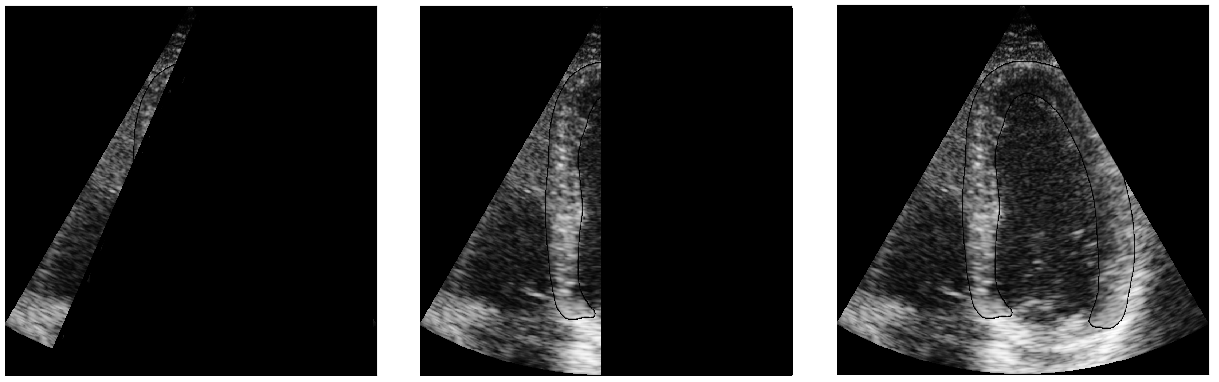
\includegraphics[width=0.99\textwidth]{echocardiography/b_mode_search.png}
    \caption{Illustration of how a two dimensional ultrasound image is put together by several individual B-mode lines. This figure is inspired by the graphical illustrations in figure 7 in \cite{basic_ultrasound}.}
    \label{fig:b_mode_search}
\end{figure}

The specific method of echocardiography used to collect the data used in this thesis is called transthoracic echocardiography. In this method ultrasound images are produced by sending ultrasound waves through the ribs of a patient, from outside the body by locating the transmitter-receiver on the chest of the patient. The transthoracic echocardiography method is constricted by the ribs such that thera are only three intersectional images that can be extracted of the heart. These three intersections are referred to as \textit{views}, and the corresponding terms are the \acrfull{4ch} view, \acrfull{2ch} view and the \acrfull{aplax} view, and examples of ultrasound images in all three views are given in figure \ref{fig:us_view_examples}.

\begin{figure}[H]
    \centering
    \begin{subfigure}[b]{0.3\textwidth} 
        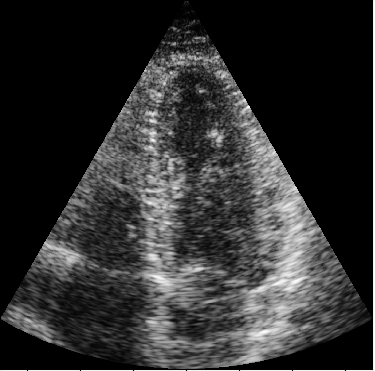
\includegraphics[width=0.99\textwidth]{echocardiography/4ch_frame.png}
        \caption{\acrshort{4ch}}
        \label{fig:us_view_examples_4ch}
    \end{subfigure}
    \begin{subfigure}[b]{0.3\textwidth}
        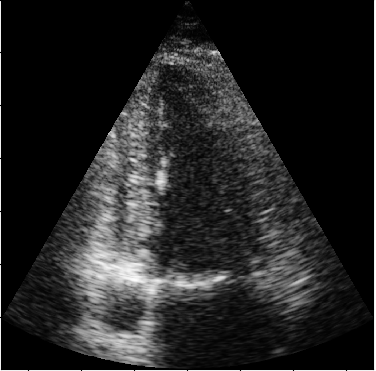
\includegraphics[width=0.99\textwidth]{echocardiography/2ch_frame.png}
        \caption{\acrshort{2ch}}
        \label{fig:us_view_examples_2ch}
    \end{subfigure}
    \begin{subfigure}[b]{0.3\textwidth}
        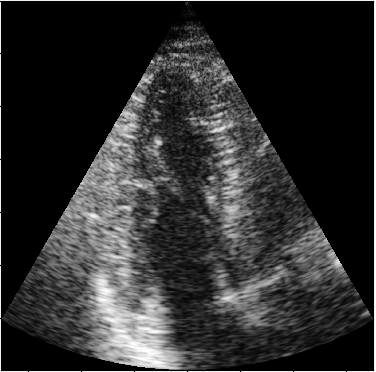
\includegraphics[width=0.99\textwidth]{echocardiography/aplax_frame.png}
        \caption{\acrshort{aplax}}
        \label{fig:us_view_examples_aplax}
    \end{subfigure}
    \caption{Examples of ultrasound images taken from the three views: (a) \acrfull{4ch}, (b) \acrfull{2ch} and (c) \acrfull{aplax}. Note that these images are flipped vertically because the ultrasound images are taken from below the heart.}
    \label{fig:us_view_examples}
\end{figure}

It is commonplace among clinicians to focus on the state of health of the left ventricle of the heart. In clinical procedure the left ventricle is divided into 16, 17 or 18 segments. This work will follow the 18-segment model, as that is the model chosen by the clinician who has annotated the images. Figure \ref{fig:18_segment_model} illustrates the 18 different segments of the left ventricle, and how they can be seen in the different views. The names of the different segments are shown in table \ref{tab:segment_names}, where the segment numbers correspond to the numbers in figure \ref{fig:18_segment_model}. When referring to the entire intersection of the left ventricle that is visible from a particular view, it will be refered to as the \textit{global segment}.

\begin{table*}
    \centering
    \ra{1}
    \begin{tabular}{cc}
        \toprule
        Segment nr. & Segment name \\
        \midrule
        1           & Basal Septal  \\
        2           & Mid Septal  \\
        3           & Apical Septal  \\
        4           & Apical Lateral  \\
        5           & Mid Lateral  \\
        6           & Basal Lateral  \\
        7           & Basal Inferior  \\
        8           & Mid Inferior  \\
        9           & Apical Inferior  \\
        10          & Apical Anterior  \\
        11          & Mid Anterior  \\
        12          & Basal Anterior  \\
        13          & Basal Posterior  \\
        14          & Mid Posterior  \\
        15          & Apical Posterior  \\
        16          & Apical Anteroseptal  \\
        17          & Mid Anteroseptal  \\
        18          & Basal Anteroseptal  \\
        \bottomrule
    \end{tabular}
    \caption{A table matching the segment numbers shown in figure \ref{fig:18_segment_model}, with the segment name.}
    \label{tab:segment_names}
\end{table*}

\begin{figure}[H]
    \centering
    \begin{subfigure}[b]{0.3\textwidth} 
        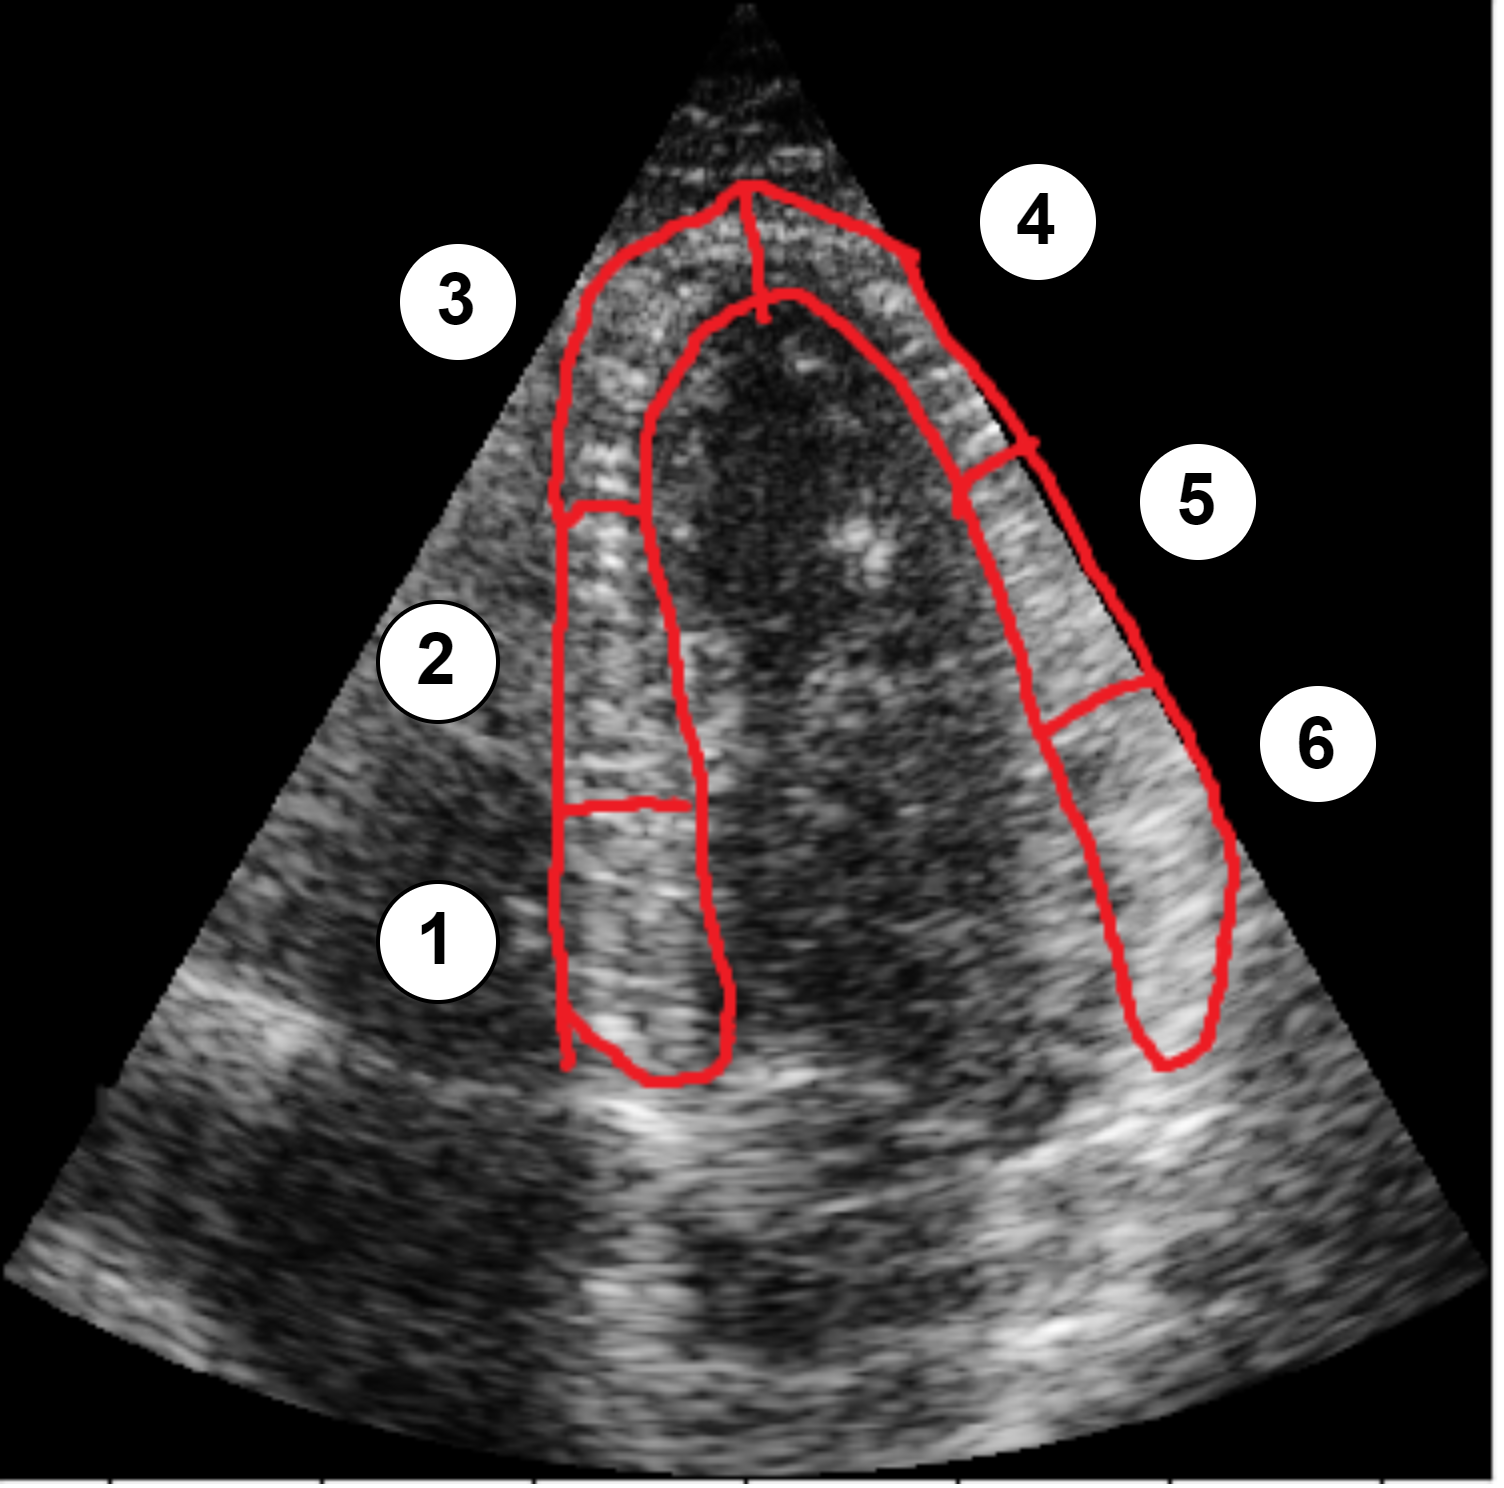
\includegraphics[width=0.99\textwidth]{echocardiography/4ch_frame_segmented.png}
        \caption{\acrshort{4ch}}
        \label{fig:18_segment_model_4ch}
    \end{subfigure}
    \begin{subfigure}[b]{0.3\textwidth}
        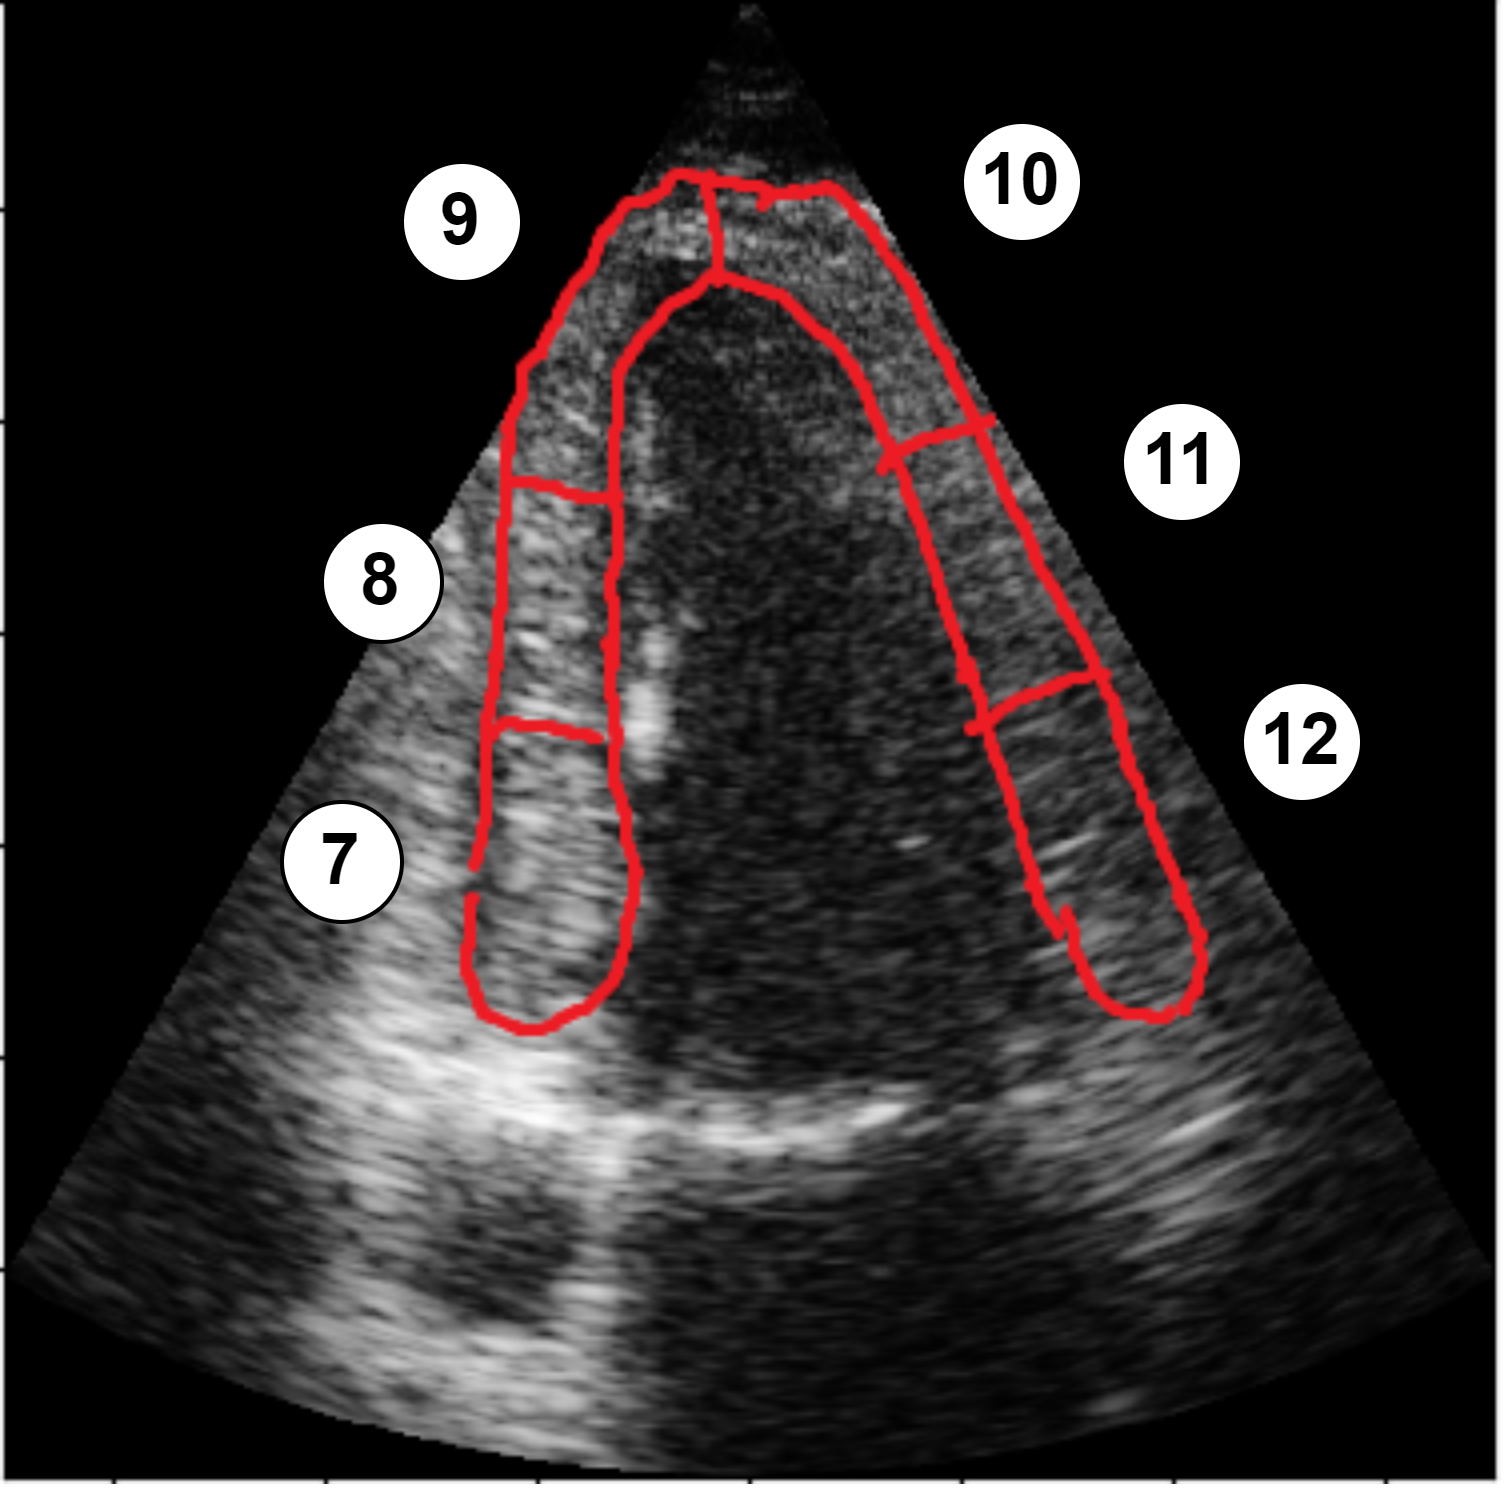
\includegraphics[width=0.99\textwidth]{echocardiography/2ch_frame_segmented.png}
        \caption{\acrshort{2ch}}
        \label{fig:18_segment_model_2ch}
    \end{subfigure}
    \begin{subfigure}[b]{0.3\textwidth}
        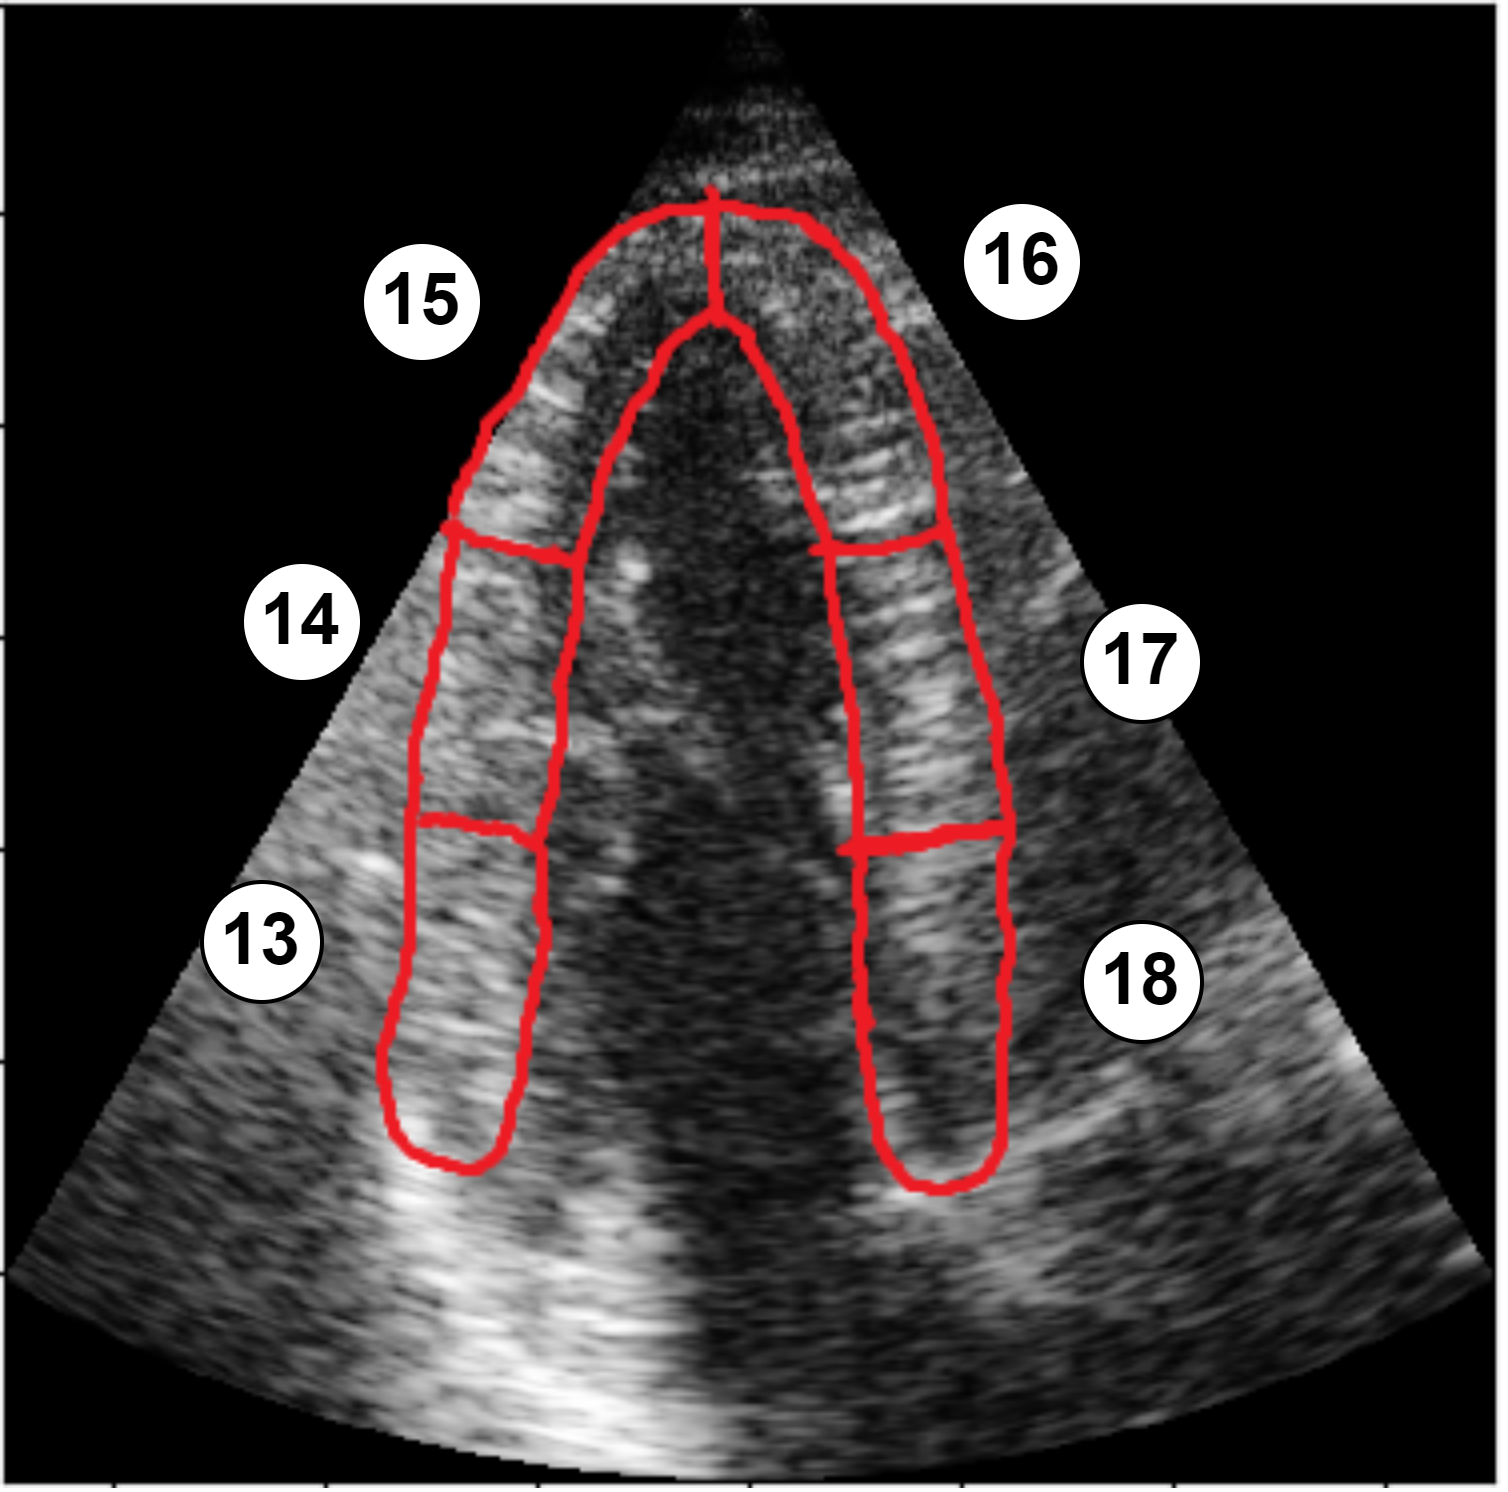
\includegraphics[width=0.99\textwidth]{echocardiography/aplax_frame_segmented.png}
        \caption{\acrshort{aplax}}
        \label{fig:18_segment_model_aplax}
    \end{subfigure}
    \caption{An illustration of the 18-segment model of the heart. It shows which segment can be seen in which view. Like in figure \ref{fig:us_view_examples} the images are flipped vertically. Note that the boundaries drawn on the figure are only meant to be illustrative, and are not the actual boundaries of the regional segments.}
    \label{fig:18_segment_model}
\end{figure}

\section{Myocardial Strain Estimation and Ejection Fraction} \label{sec:strain_est}
\begin{comment}
[ ] Method for extracting strain curves from ultrasound videos.
[ ] Examples of GLS and RLS
[ ] Define the peak systolic strain used in this work
[ ] Define Ejection fraction
\end{comment}

Strain is a relative measure of deformation, of physical objects. Since strain is relative it has no unit, and is measured in percentages in this work. The concept of strain is complex, and is well established in other scientific fields such as structural engineering. When estimating strain of linear segments, one can use the Lagrangian formula defined in \eqref{eq:linear_strain} \cite{basic_concepts}. Let $L_r$ be the length of the segment at the reference time, let $t$ be the time one wishes to measure the strain at, let the length of the segment at $t$ be denoted $L_t$ and $\epsilon(t)$ be the strain.

\begin{equation}
    \epsilon(t) = \frac{L_t - L_r}{L_r}
    \label{eq:linear_strain}
\end{equation}

This work will primarily be concerned with longitudinal strain of segments in the left ventricle. Longitudinal strain occurs due to changes in the length of a myocard segment. The two other types of strain that can be calculated with two dimensional echocardiography are transmural strain which is due to changes in the thickness of the myocard and circumferential strain which are due changes in the circumference of the entire structure \cite{basic concepts}. To estimate the strain of a particular segment, one must first define the boundaries of all the segments. There are many ways of doing this, but the most accurate method is for a clinician to draw the segment borders by hand. The clinician that annotated the dataset used in this work segmented the images using the commercial tool ECHOPAC which is developed by GE HealthCare\footnote{https://www.gehealthcare.com/products/ultrasound/vivid/echopac}. The longitudinal strain of a segment is then the relative difference in length of a segment in image frame $t$ compared to a reference image. The length of a segment is illustrated with the centerline of the vertical segment borders in figure \ref{fig:strain_estimation}. The centerline is highlighted in red in figure \ref{fig:gls_estimation}, and blue in \ref{fig:rls_estimation}. As strain is a relative measure, one needs to define a reference length which the other strain values are calculated with regard to. This could be the length of the segment during the first frame, the length of the segment when it is at its longest, the length of the segment when it is at its shortest or the length of the segment in any other ultrasound image. The strain of a segment in the reference image will then be $0\%$, and the strain of the segment in the other images will be a percentage relative to the reference image.

\begin{figure}[H]
    \centering
    \begin{subfigure}[b]{0.49\textwidth} 
        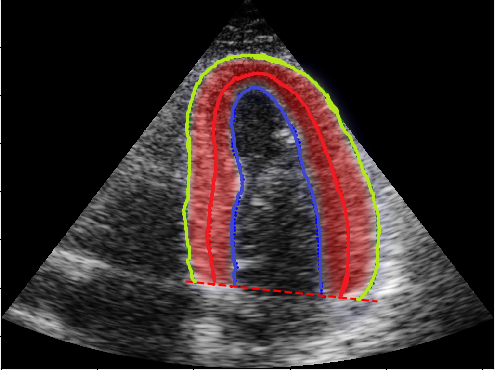
\includegraphics[width=0.99\textwidth]{echocardiography/gls_estimation.png}
        \caption{\acrshort{gls} estimation}
        \label{fig:gls_estimation}
    \end{subfigure}
    \begin{subfigure}[b]{0.49\textwidth}
        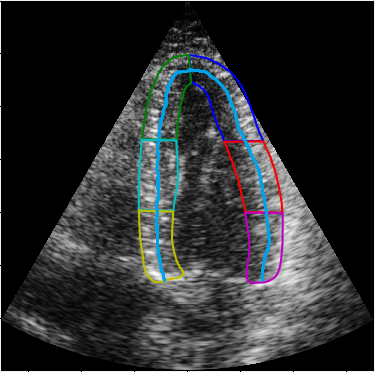
\includegraphics[width=0.99\textwidth]{echocardiography/rls_estimation.png}
        \caption{\acrshort{rls} estimation}
        \label{fig:rls_estimation}
    \end{subfigure}
    \caption{Illustration meant to assist in the understanding of what longitudinal strain is. Note that the segment borders drawn on these images are only illustrative, and are not the actual segment borders used to estimate the strain. (a) shows the strain estimation of the global segment, and (b) shows the strain estimation of the regional segments.}
    \label{fig:strain_estimation}
\end{figure}

The IMPROVE dataset included computed strain curves, but it remains unclear exactly how they were computed. There are multiple ways of computing the strain of a segment, for example the tissue Doppler and speckle tracking methods. As the name implies the the tissue Doppler method, utilizes the Doppler effect. The Doppler effect can be concisely summarized by stating that when a wave is reflected by an object that has a velocity component that is radial with regard to the direction of the wave propagation, the frequency of the reflected wave will changed with regard to the incident wave. The frequency will increase if the direction of the radial velocity component is opposite from the wave propagation direction, and it will decrease if the radial velocity component is in the same direction as the wave propagation. The magnitude of the frequency change can then be used to estimate the velocity of the moving object. Tissue Doppler then estimates the radial velocities of partitions of tissue to create a vector field of velocities \cite{strain_rate_imaging}. There are different ways of calculating strain from the velocity field, one option is to integrate the velocity field to track the displacement of the tissue partitions, but a method that requires less computation is to estimate the strain rate using equation \eqref{eq:strain_rate} \cite{myocardial_imaging}. Here $v_1$ and $v_2$ are the instantaneous velocities of the tissue partitions, and $\Delta x$ is a constant length. Strain is then estimated by integrating the strain rate over the total duration of the deformation. 

\begin{equation}
    \frac{\partial \epsilon}{\partial t} = \frac{v_2 - v_1}{\Delta x}
    \label{eq:strain_rate}
\end{equation}

The speckle tracking method is based on the fact that the spatial distribution of grey spots in an ultrasound image is inherently random. Specific regions of grey spots are referred to as speckle patterns, and each speckle pattern is unique. Since the speckle patterns are unique, their displacement can be tracked from one frame of the ultrasound video to another \cite{myocardial_imaging}. By then using the recorded longitudinal displacements of speckle patterns within a segment and equation \eqref{eq:linear_strain}, one can estimate the longitudinal strain of a segment.

By collecting all the strain values of a segment from the different ultrasound images into a time series, one gets a \textit{strain curve}. If the strain curve consists of strain values estimated from a global segment as depicted in figure \ref{fig:gls_estimation}, the curve is called a \acrfull{gls} curve. If the strain values are estimated from one of the six regional segments, as depicted in figure \ref{fig:rls_estimation}, the curves are called \acrfull{rls} curves. In diagnostic procedure it is common to extract specific values from the longitudinal strain curves. Typical strain values extracted are the peak value during the systole, the peak value during the diastole, trough values during the systole and trough values during the diastole. Figure \ref{fig:pss_illustration} shows what a typical longitudinal strain curve looks like. The peak and trough strain values during systole are illustrated by blue dots on the strain curve. The peak and trough strain values during diastole are illustrated by red dots on the strain curve. The colour shading under the curves illustrate whether the heart cycle is in systole (blue), or diastole (red). In this work one specific strain value will be tested as input data for classification models, the value that is extracted is the trough of the strain curve during the systole. This extracted strain value will be referred to as \textit{peak systolic strain}.

\begin{figure}[H]
    \centering
    %% Creator: Matplotlib, PGF backend
%%
%% To include the figure in your LaTeX document, write
%%   \input{<filename>.pgf}
%%
%% Make sure the required packages are loaded in your preamble
%%   \usepackage{pgf}
%%
%% Figures using additional raster images can only be included by \input if
%% they are in the same directory as the main LaTeX file. For loading figures
%% from other directories you can use the `import` package
%%   \usepackage{import}
%% and then include the figures with
%%   \import{<path to file>}{<filename>.pgf}
%%
%% Matplotlib used the following preamble
%%
\begingroup%
\makeatletter%
\begin{pgfpicture}%
\pgfpathrectangle{\pgfpointorigin}{\pgfqpoint{6.340000in}{2.540000in}}%
\pgfusepath{use as bounding box, clip}%
\begin{pgfscope}%
\pgfsetbuttcap%
\pgfsetmiterjoin%
\definecolor{currentfill}{rgb}{1.000000,1.000000,1.000000}%
\pgfsetfillcolor{currentfill}%
\pgfsetlinewidth{0.000000pt}%
\definecolor{currentstroke}{rgb}{1.000000,1.000000,1.000000}%
\pgfsetstrokecolor{currentstroke}%
\pgfsetdash{}{0pt}%
\pgfpathmoveto{\pgfqpoint{0.000000in}{0.000000in}}%
\pgfpathlineto{\pgfqpoint{6.340000in}{0.000000in}}%
\pgfpathlineto{\pgfqpoint{6.340000in}{2.540000in}}%
\pgfpathlineto{\pgfqpoint{0.000000in}{2.540000in}}%
\pgfpathclose%
\pgfusepath{fill}%
\end{pgfscope}%
\begin{pgfscope}%
\pgfsetbuttcap%
\pgfsetmiterjoin%
\definecolor{currentfill}{rgb}{0.917647,0.917647,0.949020}%
\pgfsetfillcolor{currentfill}%
\pgfsetlinewidth{0.000000pt}%
\definecolor{currentstroke}{rgb}{0.000000,0.000000,0.000000}%
\pgfsetstrokecolor{currentstroke}%
\pgfsetstrokeopacity{0.000000}%
\pgfsetdash{}{0pt}%
\pgfpathmoveto{\pgfqpoint{0.728470in}{0.602314in}}%
\pgfpathlineto{\pgfqpoint{6.240000in}{0.602314in}}%
\pgfpathlineto{\pgfqpoint{6.240000in}{2.440000in}}%
\pgfpathlineto{\pgfqpoint{0.728470in}{2.440000in}}%
\pgfpathclose%
\pgfusepath{fill}%
\end{pgfscope}%
\begin{pgfscope}%
\pgfpathrectangle{\pgfqpoint{0.728470in}{0.602314in}}{\pgfqpoint{5.511530in}{1.837686in}}%
\pgfusepath{clip}%
\pgfsetroundcap%
\pgfsetroundjoin%
\pgfsetlinewidth{1.003750pt}%
\definecolor{currentstroke}{rgb}{1.000000,1.000000,1.000000}%
\pgfsetstrokecolor{currentstroke}%
\pgfsetdash{}{0pt}%
\pgfpathmoveto{\pgfqpoint{0.978994in}{0.602314in}}%
\pgfpathlineto{\pgfqpoint{0.978994in}{2.440000in}}%
\pgfusepath{stroke}%
\end{pgfscope}%
\begin{pgfscope}%
\definecolor{textcolor}{rgb}{0.150000,0.150000,0.150000}%
\pgfsetstrokecolor{textcolor}%
\pgfsetfillcolor{textcolor}%
\pgftext[x=0.978994in,y=0.470370in,,top]{\color{textcolor}\sffamily\fontsize{12.000000}{14.400000}\selectfont \(\displaystyle 0.0\)}%
\end{pgfscope}%
\begin{pgfscope}%
\pgfpathrectangle{\pgfqpoint{0.728470in}{0.602314in}}{\pgfqpoint{5.511530in}{1.837686in}}%
\pgfusepath{clip}%
\pgfsetroundcap%
\pgfsetroundjoin%
\pgfsetlinewidth{1.003750pt}%
\definecolor{currentstroke}{rgb}{1.000000,1.000000,1.000000}%
\pgfsetstrokecolor{currentstroke}%
\pgfsetdash{}{0pt}%
\pgfpathmoveto{\pgfqpoint{1.620336in}{0.602314in}}%
\pgfpathlineto{\pgfqpoint{1.620336in}{2.440000in}}%
\pgfusepath{stroke}%
\end{pgfscope}%
\begin{pgfscope}%
\definecolor{textcolor}{rgb}{0.150000,0.150000,0.150000}%
\pgfsetstrokecolor{textcolor}%
\pgfsetfillcolor{textcolor}%
\pgftext[x=1.620336in,y=0.470370in,,top]{\color{textcolor}\sffamily\fontsize{12.000000}{14.400000}\selectfont \(\displaystyle 0.2\)}%
\end{pgfscope}%
\begin{pgfscope}%
\pgfpathrectangle{\pgfqpoint{0.728470in}{0.602314in}}{\pgfqpoint{5.511530in}{1.837686in}}%
\pgfusepath{clip}%
\pgfsetroundcap%
\pgfsetroundjoin%
\pgfsetlinewidth{1.003750pt}%
\definecolor{currentstroke}{rgb}{1.000000,1.000000,1.000000}%
\pgfsetstrokecolor{currentstroke}%
\pgfsetdash{}{0pt}%
\pgfpathmoveto{\pgfqpoint{2.261678in}{0.602314in}}%
\pgfpathlineto{\pgfqpoint{2.261678in}{2.440000in}}%
\pgfusepath{stroke}%
\end{pgfscope}%
\begin{pgfscope}%
\definecolor{textcolor}{rgb}{0.150000,0.150000,0.150000}%
\pgfsetstrokecolor{textcolor}%
\pgfsetfillcolor{textcolor}%
\pgftext[x=2.261678in,y=0.470370in,,top]{\color{textcolor}\sffamily\fontsize{12.000000}{14.400000}\selectfont \(\displaystyle 0.4\)}%
\end{pgfscope}%
\begin{pgfscope}%
\pgfpathrectangle{\pgfqpoint{0.728470in}{0.602314in}}{\pgfqpoint{5.511530in}{1.837686in}}%
\pgfusepath{clip}%
\pgfsetroundcap%
\pgfsetroundjoin%
\pgfsetlinewidth{1.003750pt}%
\definecolor{currentstroke}{rgb}{1.000000,1.000000,1.000000}%
\pgfsetstrokecolor{currentstroke}%
\pgfsetdash{}{0pt}%
\pgfpathmoveto{\pgfqpoint{2.903019in}{0.602314in}}%
\pgfpathlineto{\pgfqpoint{2.903019in}{2.440000in}}%
\pgfusepath{stroke}%
\end{pgfscope}%
\begin{pgfscope}%
\definecolor{textcolor}{rgb}{0.150000,0.150000,0.150000}%
\pgfsetstrokecolor{textcolor}%
\pgfsetfillcolor{textcolor}%
\pgftext[x=2.903019in,y=0.470370in,,top]{\color{textcolor}\sffamily\fontsize{12.000000}{14.400000}\selectfont \(\displaystyle 0.6\)}%
\end{pgfscope}%
\begin{pgfscope}%
\pgfpathrectangle{\pgfqpoint{0.728470in}{0.602314in}}{\pgfqpoint{5.511530in}{1.837686in}}%
\pgfusepath{clip}%
\pgfsetroundcap%
\pgfsetroundjoin%
\pgfsetlinewidth{1.003750pt}%
\definecolor{currentstroke}{rgb}{1.000000,1.000000,1.000000}%
\pgfsetstrokecolor{currentstroke}%
\pgfsetdash{}{0pt}%
\pgfpathmoveto{\pgfqpoint{3.544361in}{0.602314in}}%
\pgfpathlineto{\pgfqpoint{3.544361in}{2.440000in}}%
\pgfusepath{stroke}%
\end{pgfscope}%
\begin{pgfscope}%
\definecolor{textcolor}{rgb}{0.150000,0.150000,0.150000}%
\pgfsetstrokecolor{textcolor}%
\pgfsetfillcolor{textcolor}%
\pgftext[x=3.544361in,y=0.470370in,,top]{\color{textcolor}\sffamily\fontsize{12.000000}{14.400000}\selectfont \(\displaystyle 0.8\)}%
\end{pgfscope}%
\begin{pgfscope}%
\pgfpathrectangle{\pgfqpoint{0.728470in}{0.602314in}}{\pgfqpoint{5.511530in}{1.837686in}}%
\pgfusepath{clip}%
\pgfsetroundcap%
\pgfsetroundjoin%
\pgfsetlinewidth{1.003750pt}%
\definecolor{currentstroke}{rgb}{1.000000,1.000000,1.000000}%
\pgfsetstrokecolor{currentstroke}%
\pgfsetdash{}{0pt}%
\pgfpathmoveto{\pgfqpoint{4.185703in}{0.602314in}}%
\pgfpathlineto{\pgfqpoint{4.185703in}{2.440000in}}%
\pgfusepath{stroke}%
\end{pgfscope}%
\begin{pgfscope}%
\definecolor{textcolor}{rgb}{0.150000,0.150000,0.150000}%
\pgfsetstrokecolor{textcolor}%
\pgfsetfillcolor{textcolor}%
\pgftext[x=4.185703in,y=0.470370in,,top]{\color{textcolor}\sffamily\fontsize{12.000000}{14.400000}\selectfont \(\displaystyle 1.0\)}%
\end{pgfscope}%
\begin{pgfscope}%
\pgfpathrectangle{\pgfqpoint{0.728470in}{0.602314in}}{\pgfqpoint{5.511530in}{1.837686in}}%
\pgfusepath{clip}%
\pgfsetroundcap%
\pgfsetroundjoin%
\pgfsetlinewidth{1.003750pt}%
\definecolor{currentstroke}{rgb}{1.000000,1.000000,1.000000}%
\pgfsetstrokecolor{currentstroke}%
\pgfsetdash{}{0pt}%
\pgfpathmoveto{\pgfqpoint{4.827044in}{0.602314in}}%
\pgfpathlineto{\pgfqpoint{4.827044in}{2.440000in}}%
\pgfusepath{stroke}%
\end{pgfscope}%
\begin{pgfscope}%
\definecolor{textcolor}{rgb}{0.150000,0.150000,0.150000}%
\pgfsetstrokecolor{textcolor}%
\pgfsetfillcolor{textcolor}%
\pgftext[x=4.827044in,y=0.470370in,,top]{\color{textcolor}\sffamily\fontsize{12.000000}{14.400000}\selectfont \(\displaystyle 1.2\)}%
\end{pgfscope}%
\begin{pgfscope}%
\pgfpathrectangle{\pgfqpoint{0.728470in}{0.602314in}}{\pgfqpoint{5.511530in}{1.837686in}}%
\pgfusepath{clip}%
\pgfsetroundcap%
\pgfsetroundjoin%
\pgfsetlinewidth{1.003750pt}%
\definecolor{currentstroke}{rgb}{1.000000,1.000000,1.000000}%
\pgfsetstrokecolor{currentstroke}%
\pgfsetdash{}{0pt}%
\pgfpathmoveto{\pgfqpoint{5.468386in}{0.602314in}}%
\pgfpathlineto{\pgfqpoint{5.468386in}{2.440000in}}%
\pgfusepath{stroke}%
\end{pgfscope}%
\begin{pgfscope}%
\definecolor{textcolor}{rgb}{0.150000,0.150000,0.150000}%
\pgfsetstrokecolor{textcolor}%
\pgfsetfillcolor{textcolor}%
\pgftext[x=5.468386in,y=0.470370in,,top]{\color{textcolor}\sffamily\fontsize{12.000000}{14.400000}\selectfont \(\displaystyle 1.4\)}%
\end{pgfscope}%
\begin{pgfscope}%
\pgfpathrectangle{\pgfqpoint{0.728470in}{0.602314in}}{\pgfqpoint{5.511530in}{1.837686in}}%
\pgfusepath{clip}%
\pgfsetroundcap%
\pgfsetroundjoin%
\pgfsetlinewidth{1.003750pt}%
\definecolor{currentstroke}{rgb}{1.000000,1.000000,1.000000}%
\pgfsetstrokecolor{currentstroke}%
\pgfsetdash{}{0pt}%
\pgfpathmoveto{\pgfqpoint{6.109727in}{0.602314in}}%
\pgfpathlineto{\pgfqpoint{6.109727in}{2.440000in}}%
\pgfusepath{stroke}%
\end{pgfscope}%
\begin{pgfscope}%
\definecolor{textcolor}{rgb}{0.150000,0.150000,0.150000}%
\pgfsetstrokecolor{textcolor}%
\pgfsetfillcolor{textcolor}%
\pgftext[x=6.109727in,y=0.470370in,,top]{\color{textcolor}\sffamily\fontsize{12.000000}{14.400000}\selectfont \(\displaystyle 1.6\)}%
\end{pgfscope}%
\begin{pgfscope}%
\definecolor{textcolor}{rgb}{0.150000,0.150000,0.150000}%
\pgfsetstrokecolor{textcolor}%
\pgfsetfillcolor{textcolor}%
\pgftext[x=3.484235in,y=0.266667in,,top]{\color{textcolor}\sffamily\fontsize{12.000000}{14.400000}\selectfont Time [s]}%
\end{pgfscope}%
\begin{pgfscope}%
\pgfpathrectangle{\pgfqpoint{0.728470in}{0.602314in}}{\pgfqpoint{5.511530in}{1.837686in}}%
\pgfusepath{clip}%
\pgfsetroundcap%
\pgfsetroundjoin%
\pgfsetlinewidth{1.003750pt}%
\definecolor{currentstroke}{rgb}{1.000000,1.000000,1.000000}%
\pgfsetstrokecolor{currentstroke}%
\pgfsetdash{}{0pt}%
\pgfpathmoveto{\pgfqpoint{0.728470in}{1.105106in}}%
\pgfpathlineto{\pgfqpoint{6.240000in}{1.105106in}}%
\pgfusepath{stroke}%
\end{pgfscope}%
\begin{pgfscope}%
\definecolor{textcolor}{rgb}{0.150000,0.150000,0.150000}%
\pgfsetstrokecolor{textcolor}%
\pgfsetfillcolor{textcolor}%
\pgftext[x=0.303703in,y=1.047235in,left,base]{\color{textcolor}\sffamily\fontsize{12.000000}{14.400000}\selectfont \(\displaystyle -10\)}%
\end{pgfscope}%
\begin{pgfscope}%
\pgfpathrectangle{\pgfqpoint{0.728470in}{0.602314in}}{\pgfqpoint{5.511530in}{1.837686in}}%
\pgfusepath{clip}%
\pgfsetroundcap%
\pgfsetroundjoin%
\pgfsetlinewidth{1.003750pt}%
\definecolor{currentstroke}{rgb}{1.000000,1.000000,1.000000}%
\pgfsetstrokecolor{currentstroke}%
\pgfsetdash{}{0pt}%
\pgfpathmoveto{\pgfqpoint{0.728470in}{1.704049in}}%
\pgfpathlineto{\pgfqpoint{6.240000in}{1.704049in}}%
\pgfusepath{stroke}%
\end{pgfscope}%
\begin{pgfscope}%
\definecolor{textcolor}{rgb}{0.150000,0.150000,0.150000}%
\pgfsetstrokecolor{textcolor}%
\pgfsetfillcolor{textcolor}%
\pgftext[x=0.385299in,y=1.646179in,left,base]{\color{textcolor}\sffamily\fontsize{12.000000}{14.400000}\selectfont \(\displaystyle -5\)}%
\end{pgfscope}%
\begin{pgfscope}%
\pgfpathrectangle{\pgfqpoint{0.728470in}{0.602314in}}{\pgfqpoint{5.511530in}{1.837686in}}%
\pgfusepath{clip}%
\pgfsetroundcap%
\pgfsetroundjoin%
\pgfsetlinewidth{1.003750pt}%
\definecolor{currentstroke}{rgb}{1.000000,1.000000,1.000000}%
\pgfsetstrokecolor{currentstroke}%
\pgfsetdash{}{0pt}%
\pgfpathmoveto{\pgfqpoint{0.728470in}{2.302992in}}%
\pgfpathlineto{\pgfqpoint{6.240000in}{2.302992in}}%
\pgfusepath{stroke}%
\end{pgfscope}%
\begin{pgfscope}%
\definecolor{textcolor}{rgb}{0.150000,0.150000,0.150000}%
\pgfsetstrokecolor{textcolor}%
\pgfsetfillcolor{textcolor}%
\pgftext[x=0.514929in,y=2.245122in,left,base]{\color{textcolor}\sffamily\fontsize{12.000000}{14.400000}\selectfont \(\displaystyle 0\)}%
\end{pgfscope}%
\begin{pgfscope}%
\definecolor{textcolor}{rgb}{0.150000,0.150000,0.150000}%
\pgfsetstrokecolor{textcolor}%
\pgfsetfillcolor{textcolor}%
\pgftext[x=0.248148in,y=1.521157in,,bottom,rotate=90.000000]{\color{textcolor}\sffamily\fontsize{12.000000}{14.400000}\selectfont Strain}%
\end{pgfscope}%
\begin{pgfscope}%
\pgfpathrectangle{\pgfqpoint{0.728470in}{0.602314in}}{\pgfqpoint{5.511530in}{1.837686in}}%
\pgfusepath{clip}%
\pgfsetbuttcap%
\pgfsetroundjoin%
\definecolor{currentfill}{rgb}{0.298039,0.447059,0.690196}%
\pgfsetfillcolor{currentfill}%
\pgfsetfillopacity{0.300000}%
\pgfsetlinewidth{1.003750pt}%
\definecolor{currentstroke}{rgb}{0.298039,0.447059,0.690196}%
\pgfsetstrokecolor{currentstroke}%
\pgfsetstrokeopacity{0.300000}%
\pgfsetdash{}{0pt}%
\pgfpathmoveto{\pgfqpoint{0.978994in}{1.962271in}}%
\pgfpathlineto{\pgfqpoint{0.978994in}{0.685845in}}%
\pgfpathlineto{\pgfqpoint{1.029099in}{0.685845in}}%
\pgfpathlineto{\pgfqpoint{1.079204in}{0.685845in}}%
\pgfpathlineto{\pgfqpoint{1.129309in}{0.685845in}}%
\pgfpathlineto{\pgfqpoint{1.179414in}{0.685845in}}%
\pgfpathlineto{\pgfqpoint{1.229518in}{0.685845in}}%
\pgfpathlineto{\pgfqpoint{1.279623in}{0.685845in}}%
\pgfpathlineto{\pgfqpoint{1.329728in}{0.685845in}}%
\pgfpathlineto{\pgfqpoint{1.379833in}{0.685845in}}%
\pgfpathlineto{\pgfqpoint{1.429938in}{0.685845in}}%
\pgfpathlineto{\pgfqpoint{1.480043in}{0.685845in}}%
\pgfpathlineto{\pgfqpoint{1.530147in}{0.685845in}}%
\pgfpathlineto{\pgfqpoint{1.580252in}{0.685845in}}%
\pgfpathlineto{\pgfqpoint{1.630357in}{0.685845in}}%
\pgfpathlineto{\pgfqpoint{1.680462in}{0.685845in}}%
\pgfpathlineto{\pgfqpoint{1.730567in}{0.685845in}}%
\pgfpathlineto{\pgfqpoint{1.780671in}{0.685845in}}%
\pgfpathlineto{\pgfqpoint{1.830776in}{0.685845in}}%
\pgfpathlineto{\pgfqpoint{1.880881in}{0.685845in}}%
\pgfpathlineto{\pgfqpoint{1.930986in}{0.685845in}}%
\pgfpathlineto{\pgfqpoint{1.981091in}{0.685845in}}%
\pgfpathlineto{\pgfqpoint{2.031195in}{0.685845in}}%
\pgfpathlineto{\pgfqpoint{2.081300in}{0.685845in}}%
\pgfpathlineto{\pgfqpoint{2.131405in}{0.685845in}}%
\pgfpathlineto{\pgfqpoint{2.181510in}{0.685845in}}%
\pgfpathlineto{\pgfqpoint{2.231615in}{0.685845in}}%
\pgfpathlineto{\pgfqpoint{2.281720in}{0.685845in}}%
\pgfpathlineto{\pgfqpoint{2.331824in}{0.685845in}}%
\pgfpathlineto{\pgfqpoint{2.381929in}{0.685845in}}%
\pgfpathlineto{\pgfqpoint{2.432034in}{0.685845in}}%
\pgfpathlineto{\pgfqpoint{2.482139in}{0.685845in}}%
\pgfpathlineto{\pgfqpoint{2.532244in}{0.685845in}}%
\pgfpathlineto{\pgfqpoint{2.582348in}{0.685845in}}%
\pgfpathlineto{\pgfqpoint{2.632453in}{0.685845in}}%
\pgfpathlineto{\pgfqpoint{2.682558in}{0.685845in}}%
\pgfpathlineto{\pgfqpoint{2.732663in}{0.685845in}}%
\pgfpathlineto{\pgfqpoint{2.782768in}{0.685845in}}%
\pgfpathlineto{\pgfqpoint{2.832873in}{0.685845in}}%
\pgfpathlineto{\pgfqpoint{2.882977in}{0.685845in}}%
\pgfpathlineto{\pgfqpoint{2.933082in}{0.685845in}}%
\pgfpathlineto{\pgfqpoint{2.983187in}{0.685845in}}%
\pgfpathlineto{\pgfqpoint{3.033292in}{0.685845in}}%
\pgfpathlineto{\pgfqpoint{3.083397in}{0.685845in}}%
\pgfpathlineto{\pgfqpoint{3.133501in}{0.685845in}}%
\pgfpathlineto{\pgfqpoint{3.183606in}{0.685845in}}%
\pgfpathlineto{\pgfqpoint{3.183606in}{0.811826in}}%
\pgfpathlineto{\pgfqpoint{3.183606in}{0.811826in}}%
\pgfpathlineto{\pgfqpoint{3.133501in}{0.783501in}}%
\pgfpathlineto{\pgfqpoint{3.083397in}{0.774631in}}%
\pgfpathlineto{\pgfqpoint{3.033292in}{0.769909in}}%
\pgfpathlineto{\pgfqpoint{2.983187in}{0.763368in}}%
\pgfpathlineto{\pgfqpoint{2.933082in}{0.755592in}}%
\pgfpathlineto{\pgfqpoint{2.882977in}{0.748173in}}%
\pgfpathlineto{\pgfqpoint{2.832873in}{0.740620in}}%
\pgfpathlineto{\pgfqpoint{2.782768in}{0.731824in}}%
\pgfpathlineto{\pgfqpoint{2.732663in}{0.723730in}}%
\pgfpathlineto{\pgfqpoint{2.682558in}{0.722012in}}%
\pgfpathlineto{\pgfqpoint{2.632453in}{0.733274in}}%
\pgfpathlineto{\pgfqpoint{2.582348in}{0.761881in}}%
\pgfpathlineto{\pgfqpoint{2.532244in}{0.807844in}}%
\pgfpathlineto{\pgfqpoint{2.482139in}{0.866719in}}%
\pgfpathlineto{\pgfqpoint{2.432034in}{0.934317in}}%
\pgfpathlineto{\pgfqpoint{2.381929in}{1.010635in}}%
\pgfpathlineto{\pgfqpoint{2.331824in}{1.100265in}}%
\pgfpathlineto{\pgfqpoint{2.281720in}{1.208523in}}%
\pgfpathlineto{\pgfqpoint{2.231615in}{1.334555in}}%
\pgfpathlineto{\pgfqpoint{2.181510in}{1.469757in}}%
\pgfpathlineto{\pgfqpoint{2.131405in}{1.605028in}}%
\pgfpathlineto{\pgfqpoint{2.081300in}{1.736193in}}%
\pgfpathlineto{\pgfqpoint{2.031195in}{1.860088in}}%
\pgfpathlineto{\pgfqpoint{1.981091in}{1.971364in}}%
\pgfpathlineto{\pgfqpoint{1.930986in}{2.066555in}}%
\pgfpathlineto{\pgfqpoint{1.880881in}{2.145999in}}%
\pgfpathlineto{\pgfqpoint{1.830776in}{2.211525in}}%
\pgfpathlineto{\pgfqpoint{1.780671in}{2.260978in}}%
\pgfpathlineto{\pgfqpoint{1.730567in}{2.291380in}}%
\pgfpathlineto{\pgfqpoint{1.680462in}{2.302992in}}%
\pgfpathlineto{\pgfqpoint{1.630357in}{2.301584in}}%
\pgfpathlineto{\pgfqpoint{1.580252in}{2.292281in}}%
\pgfpathlineto{\pgfqpoint{1.530147in}{2.272969in}}%
\pgfpathlineto{\pgfqpoint{1.480043in}{2.235568in}}%
\pgfpathlineto{\pgfqpoint{1.429938in}{2.176100in}}%
\pgfpathlineto{\pgfqpoint{1.379833in}{2.103664in}}%
\pgfpathlineto{\pgfqpoint{1.329728in}{2.037376in}}%
\pgfpathlineto{\pgfqpoint{1.279623in}{1.991957in}}%
\pgfpathlineto{\pgfqpoint{1.229518in}{1.968768in}}%
\pgfpathlineto{\pgfqpoint{1.179414in}{1.960291in}}%
\pgfpathlineto{\pgfqpoint{1.129309in}{1.958907in}}%
\pgfpathlineto{\pgfqpoint{1.079204in}{1.959958in}}%
\pgfpathlineto{\pgfqpoint{1.029099in}{1.961253in}}%
\pgfpathlineto{\pgfqpoint{0.978994in}{1.962271in}}%
\pgfpathclose%
\pgfusepath{stroke,fill}%
\end{pgfscope}%
\begin{pgfscope}%
\pgfpathrectangle{\pgfqpoint{0.728470in}{0.602314in}}{\pgfqpoint{5.511530in}{1.837686in}}%
\pgfusepath{clip}%
\pgfsetbuttcap%
\pgfsetroundjoin%
\definecolor{currentfill}{rgb}{0.768627,0.305882,0.321569}%
\pgfsetfillcolor{currentfill}%
\pgfsetfillopacity{0.300000}%
\pgfsetlinewidth{1.003750pt}%
\definecolor{currentstroke}{rgb}{0.768627,0.305882,0.321569}%
\pgfsetstrokecolor{currentstroke}%
\pgfsetstrokeopacity{0.300000}%
\pgfsetdash{}{0pt}%
\pgfpathmoveto{\pgfqpoint{3.233711in}{0.878046in}}%
\pgfpathlineto{\pgfqpoint{3.233711in}{0.685845in}}%
\pgfpathlineto{\pgfqpoint{3.283816in}{0.685845in}}%
\pgfpathlineto{\pgfqpoint{3.333921in}{0.685845in}}%
\pgfpathlineto{\pgfqpoint{3.384026in}{0.685845in}}%
\pgfpathlineto{\pgfqpoint{3.434130in}{0.685845in}}%
\pgfpathlineto{\pgfqpoint{3.484235in}{0.685845in}}%
\pgfpathlineto{\pgfqpoint{3.534340in}{0.685845in}}%
\pgfpathlineto{\pgfqpoint{3.584445in}{0.685845in}}%
\pgfpathlineto{\pgfqpoint{3.634550in}{0.685845in}}%
\pgfpathlineto{\pgfqpoint{3.684654in}{0.685845in}}%
\pgfpathlineto{\pgfqpoint{3.734759in}{0.685845in}}%
\pgfpathlineto{\pgfqpoint{3.784864in}{0.685845in}}%
\pgfpathlineto{\pgfqpoint{3.834969in}{0.685845in}}%
\pgfpathlineto{\pgfqpoint{3.885074in}{0.685845in}}%
\pgfpathlineto{\pgfqpoint{3.935178in}{0.685845in}}%
\pgfpathlineto{\pgfqpoint{3.985283in}{0.685845in}}%
\pgfpathlineto{\pgfqpoint{4.035388in}{0.685845in}}%
\pgfpathlineto{\pgfqpoint{4.085493in}{0.685845in}}%
\pgfpathlineto{\pgfqpoint{4.135598in}{0.685845in}}%
\pgfpathlineto{\pgfqpoint{4.185703in}{0.685845in}}%
\pgfpathlineto{\pgfqpoint{4.235807in}{0.685845in}}%
\pgfpathlineto{\pgfqpoint{4.285912in}{0.685845in}}%
\pgfpathlineto{\pgfqpoint{4.336017in}{0.685845in}}%
\pgfpathlineto{\pgfqpoint{4.386122in}{0.685845in}}%
\pgfpathlineto{\pgfqpoint{4.436227in}{0.685845in}}%
\pgfpathlineto{\pgfqpoint{4.486331in}{0.685845in}}%
\pgfpathlineto{\pgfqpoint{4.536436in}{0.685845in}}%
\pgfpathlineto{\pgfqpoint{4.586541in}{0.685845in}}%
\pgfpathlineto{\pgfqpoint{4.636646in}{0.685845in}}%
\pgfpathlineto{\pgfqpoint{4.686751in}{0.685845in}}%
\pgfpathlineto{\pgfqpoint{4.736856in}{0.685845in}}%
\pgfpathlineto{\pgfqpoint{4.786960in}{0.685845in}}%
\pgfpathlineto{\pgfqpoint{4.837065in}{0.685845in}}%
\pgfpathlineto{\pgfqpoint{4.887170in}{0.685845in}}%
\pgfpathlineto{\pgfqpoint{4.937275in}{0.685845in}}%
\pgfpathlineto{\pgfqpoint{4.987380in}{0.685845in}}%
\pgfpathlineto{\pgfqpoint{5.037484in}{0.685845in}}%
\pgfpathlineto{\pgfqpoint{5.087589in}{0.685845in}}%
\pgfpathlineto{\pgfqpoint{5.137694in}{0.685845in}}%
\pgfpathlineto{\pgfqpoint{5.187799in}{0.685845in}}%
\pgfpathlineto{\pgfqpoint{5.237904in}{0.685845in}}%
\pgfpathlineto{\pgfqpoint{5.288009in}{0.685845in}}%
\pgfpathlineto{\pgfqpoint{5.338113in}{0.685845in}}%
\pgfpathlineto{\pgfqpoint{5.388218in}{0.685845in}}%
\pgfpathlineto{\pgfqpoint{5.438323in}{0.685845in}}%
\pgfpathlineto{\pgfqpoint{5.488428in}{0.685845in}}%
\pgfpathlineto{\pgfqpoint{5.538533in}{0.685845in}}%
\pgfpathlineto{\pgfqpoint{5.588637in}{0.685845in}}%
\pgfpathlineto{\pgfqpoint{5.638742in}{0.685845in}}%
\pgfpathlineto{\pgfqpoint{5.688847in}{0.685845in}}%
\pgfpathlineto{\pgfqpoint{5.738952in}{0.685845in}}%
\pgfpathlineto{\pgfqpoint{5.789057in}{0.685845in}}%
\pgfpathlineto{\pgfqpoint{5.839161in}{0.685845in}}%
\pgfpathlineto{\pgfqpoint{5.889266in}{0.685845in}}%
\pgfpathlineto{\pgfqpoint{5.939371in}{0.685845in}}%
\pgfpathlineto{\pgfqpoint{5.989476in}{0.685845in}}%
\pgfpathlineto{\pgfqpoint{5.989476in}{0.707198in}}%
\pgfpathlineto{\pgfqpoint{5.989476in}{0.707198in}}%
\pgfpathlineto{\pgfqpoint{5.939371in}{0.818465in}}%
\pgfpathlineto{\pgfqpoint{5.889266in}{0.943302in}}%
\pgfpathlineto{\pgfqpoint{5.839161in}{1.082254in}}%
\pgfpathlineto{\pgfqpoint{5.789057in}{1.226614in}}%
\pgfpathlineto{\pgfqpoint{5.738952in}{1.369412in}}%
\pgfpathlineto{\pgfqpoint{5.688847in}{1.508296in}}%
\pgfpathlineto{\pgfqpoint{5.638742in}{1.642391in}}%
\pgfpathlineto{\pgfqpoint{5.588637in}{1.771733in}}%
\pgfpathlineto{\pgfqpoint{5.538533in}{1.896957in}}%
\pgfpathlineto{\pgfqpoint{5.488428in}{2.016190in}}%
\pgfpathlineto{\pgfqpoint{5.438323in}{2.122016in}}%
\pgfpathlineto{\pgfqpoint{5.388218in}{2.206623in}}%
\pgfpathlineto{\pgfqpoint{5.338113in}{2.266566in}}%
\pgfpathlineto{\pgfqpoint{5.288009in}{2.302992in}}%
\pgfpathlineto{\pgfqpoint{5.237904in}{2.319213in}}%
\pgfpathlineto{\pgfqpoint{5.187799in}{2.319285in}}%
\pgfpathlineto{\pgfqpoint{5.137694in}{2.306209in}}%
\pgfpathlineto{\pgfqpoint{5.087589in}{2.281027in}}%
\pgfpathlineto{\pgfqpoint{5.037484in}{2.244337in}}%
\pgfpathlineto{\pgfqpoint{4.987380in}{2.199168in}}%
\pgfpathlineto{\pgfqpoint{4.937275in}{2.152361in}}%
\pgfpathlineto{\pgfqpoint{4.887170in}{2.111916in}}%
\pgfpathlineto{\pgfqpoint{4.837065in}{2.083609in}}%
\pgfpathlineto{\pgfqpoint{4.786960in}{2.067567in}}%
\pgfpathlineto{\pgfqpoint{4.736856in}{2.059242in}}%
\pgfpathlineto{\pgfqpoint{4.686751in}{2.053593in}}%
\pgfpathlineto{\pgfqpoint{4.636646in}{2.048548in}}%
\pgfpathlineto{\pgfqpoint{4.586541in}{2.045927in}}%
\pgfpathlineto{\pgfqpoint{4.536436in}{2.048988in}}%
\pgfpathlineto{\pgfqpoint{4.486331in}{2.058466in}}%
\pgfpathlineto{\pgfqpoint{4.436227in}{2.071259in}}%
\pgfpathlineto{\pgfqpoint{4.386122in}{2.084171in}}%
\pgfpathlineto{\pgfqpoint{4.336017in}{2.094204in}}%
\pgfpathlineto{\pgfqpoint{4.285912in}{2.097947in}}%
\pgfpathlineto{\pgfqpoint{4.235807in}{2.093268in}}%
\pgfpathlineto{\pgfqpoint{4.185703in}{2.081157in}}%
\pgfpathlineto{\pgfqpoint{4.135598in}{2.065135in}}%
\pgfpathlineto{\pgfqpoint{4.085493in}{2.049862in}}%
\pgfpathlineto{\pgfqpoint{4.035388in}{2.037498in}}%
\pgfpathlineto{\pgfqpoint{3.985283in}{2.025406in}}%
\pgfpathlineto{\pgfqpoint{3.935178in}{2.009822in}}%
\pgfpathlineto{\pgfqpoint{3.885074in}{1.989775in}}%
\pgfpathlineto{\pgfqpoint{3.834969in}{1.966943in}}%
\pgfpathlineto{\pgfqpoint{3.784864in}{1.942162in}}%
\pgfpathlineto{\pgfqpoint{3.734759in}{1.913614in}}%
\pgfpathlineto{\pgfqpoint{3.684654in}{1.878509in}}%
\pgfpathlineto{\pgfqpoint{3.634550in}{1.835439in}}%
\pgfpathlineto{\pgfqpoint{3.584445in}{1.782422in}}%
\pgfpathlineto{\pgfqpoint{3.534340in}{1.711764in}}%
\pgfpathlineto{\pgfqpoint{3.484235in}{1.612455in}}%
\pgfpathlineto{\pgfqpoint{3.434130in}{1.478411in}}%
\pgfpathlineto{\pgfqpoint{3.384026in}{1.315684in}}%
\pgfpathlineto{\pgfqpoint{3.333921in}{1.144256in}}%
\pgfpathlineto{\pgfqpoint{3.283816in}{0.991193in}}%
\pgfpathlineto{\pgfqpoint{3.233711in}{0.878046in}}%
\pgfpathclose%
\pgfusepath{stroke,fill}%
\end{pgfscope}%
\begin{pgfscope}%
\pgfpathrectangle{\pgfqpoint{0.728470in}{0.602314in}}{\pgfqpoint{5.511530in}{1.837686in}}%
\pgfusepath{clip}%
\pgfsetbuttcap%
\pgfsetroundjoin%
\definecolor{currentfill}{rgb}{0.298039,0.447059,0.690196}%
\pgfsetfillcolor{currentfill}%
\pgfsetlinewidth{1.003750pt}%
\definecolor{currentstroke}{rgb}{0.298039,0.447059,0.690196}%
\pgfsetstrokecolor{currentstroke}%
\pgfsetdash{}{0pt}%
\pgfpathmoveto{\pgfqpoint{1.680462in}{2.261325in}}%
\pgfpathcurveto{\pgfqpoint{1.691512in}{2.261325in}}{\pgfqpoint{1.702111in}{2.265716in}}{\pgfqpoint{1.709925in}{2.273529in}}%
\pgfpathcurveto{\pgfqpoint{1.717738in}{2.281343in}}{\pgfqpoint{1.722128in}{2.291942in}}{\pgfqpoint{1.722128in}{2.302992in}}%
\pgfpathcurveto{\pgfqpoint{1.722128in}{2.314042in}}{\pgfqpoint{1.717738in}{2.324641in}}{\pgfqpoint{1.709925in}{2.332455in}}%
\pgfpathcurveto{\pgfqpoint{1.702111in}{2.340269in}}{\pgfqpoint{1.691512in}{2.344659in}}{\pgfqpoint{1.680462in}{2.344659in}}%
\pgfpathcurveto{\pgfqpoint{1.669412in}{2.344659in}}{\pgfqpoint{1.658813in}{2.340269in}}{\pgfqpoint{1.650999in}{2.332455in}}%
\pgfpathcurveto{\pgfqpoint{1.643185in}{2.324641in}}{\pgfqpoint{1.638795in}{2.314042in}}{\pgfqpoint{1.638795in}{2.302992in}}%
\pgfpathcurveto{\pgfqpoint{1.638795in}{2.291942in}}{\pgfqpoint{1.643185in}{2.281343in}}{\pgfqpoint{1.650999in}{2.273529in}}%
\pgfpathcurveto{\pgfqpoint{1.658813in}{2.265716in}}{\pgfqpoint{1.669412in}{2.261325in}}{\pgfqpoint{1.680462in}{2.261325in}}%
\pgfpathclose%
\pgfusepath{stroke,fill}%
\end{pgfscope}%
\begin{pgfscope}%
\pgfpathrectangle{\pgfqpoint{0.728470in}{0.602314in}}{\pgfqpoint{5.511530in}{1.837686in}}%
\pgfusepath{clip}%
\pgfsetbuttcap%
\pgfsetroundjoin%
\definecolor{currentfill}{rgb}{0.298039,0.447059,0.690196}%
\pgfsetfillcolor{currentfill}%
\pgfsetlinewidth{1.003750pt}%
\definecolor{currentstroke}{rgb}{0.298039,0.447059,0.690196}%
\pgfsetstrokecolor{currentstroke}%
\pgfsetdash{}{0pt}%
\pgfpathmoveto{\pgfqpoint{2.682558in}{0.692094in}}%
\pgfpathcurveto{\pgfqpoint{2.693608in}{0.692094in}}{\pgfqpoint{2.704207in}{0.696484in}}{\pgfqpoint{2.712021in}{0.704298in}}%
\pgfpathcurveto{\pgfqpoint{2.719834in}{0.712112in}}{\pgfqpoint{2.724225in}{0.722711in}}{\pgfqpoint{2.724225in}{0.733761in}}%
\pgfpathcurveto{\pgfqpoint{2.724225in}{0.744811in}}{\pgfqpoint{2.719834in}{0.755410in}}{\pgfqpoint{2.712021in}{0.763224in}}%
\pgfpathcurveto{\pgfqpoint{2.704207in}{0.771037in}}{\pgfqpoint{2.693608in}{0.775427in}}{\pgfqpoint{2.682558in}{0.775427in}}%
\pgfpathcurveto{\pgfqpoint{2.671508in}{0.775427in}}{\pgfqpoint{2.660909in}{0.771037in}}{\pgfqpoint{2.653095in}{0.763224in}}%
\pgfpathcurveto{\pgfqpoint{2.645282in}{0.755410in}}{\pgfqpoint{2.640891in}{0.744811in}}{\pgfqpoint{2.640891in}{0.733761in}}%
\pgfpathcurveto{\pgfqpoint{2.640891in}{0.722711in}}{\pgfqpoint{2.645282in}{0.712112in}}{\pgfqpoint{2.653095in}{0.704298in}}%
\pgfpathcurveto{\pgfqpoint{2.660909in}{0.696484in}}{\pgfqpoint{2.671508in}{0.692094in}}{\pgfqpoint{2.682558in}{0.692094in}}%
\pgfpathclose%
\pgfusepath{stroke,fill}%
\end{pgfscope}%
\begin{pgfscope}%
\pgfpathrectangle{\pgfqpoint{0.728470in}{0.602314in}}{\pgfqpoint{5.511530in}{1.837686in}}%
\pgfusepath{clip}%
\pgfsetbuttcap%
\pgfsetroundjoin%
\definecolor{currentfill}{rgb}{0.768627,0.305882,0.321569}%
\pgfsetfillcolor{currentfill}%
\pgfsetlinewidth{1.003750pt}%
\definecolor{currentstroke}{rgb}{0.768627,0.305882,0.321569}%
\pgfsetstrokecolor{currentstroke}%
\pgfsetdash{}{0pt}%
\pgfpathmoveto{\pgfqpoint{3.233711in}{0.836380in}}%
\pgfpathcurveto{\pgfqpoint{3.244761in}{0.836380in}}{\pgfqpoint{3.255360in}{0.840770in}}{\pgfqpoint{3.263174in}{0.848583in}}%
\pgfpathcurveto{\pgfqpoint{3.270987in}{0.856397in}}{\pgfqpoint{3.275378in}{0.866996in}}{\pgfqpoint{3.275378in}{0.878046in}}%
\pgfpathcurveto{\pgfqpoint{3.275378in}{0.889096in}}{\pgfqpoint{3.270987in}{0.899695in}}{\pgfqpoint{3.263174in}{0.907509in}}%
\pgfpathcurveto{\pgfqpoint{3.255360in}{0.915323in}}{\pgfqpoint{3.244761in}{0.919713in}}{\pgfqpoint{3.233711in}{0.919713in}}%
\pgfpathcurveto{\pgfqpoint{3.222661in}{0.919713in}}{\pgfqpoint{3.212062in}{0.915323in}}{\pgfqpoint{3.204248in}{0.907509in}}%
\pgfpathcurveto{\pgfqpoint{3.196435in}{0.899695in}}{\pgfqpoint{3.192044in}{0.889096in}}{\pgfqpoint{3.192044in}{0.878046in}}%
\pgfpathcurveto{\pgfqpoint{3.192044in}{0.866996in}}{\pgfqpoint{3.196435in}{0.856397in}}{\pgfqpoint{3.204248in}{0.848583in}}%
\pgfpathcurveto{\pgfqpoint{3.212062in}{0.840770in}}{\pgfqpoint{3.222661in}{0.836380in}}{\pgfqpoint{3.233711in}{0.836380in}}%
\pgfpathclose%
\pgfusepath{stroke,fill}%
\end{pgfscope}%
\begin{pgfscope}%
\pgfpathrectangle{\pgfqpoint{0.728470in}{0.602314in}}{\pgfqpoint{5.511530in}{1.837686in}}%
\pgfusepath{clip}%
\pgfsetbuttcap%
\pgfsetroundjoin%
\definecolor{currentfill}{rgb}{0.768627,0.305882,0.321569}%
\pgfsetfillcolor{currentfill}%
\pgfsetlinewidth{1.003750pt}%
\definecolor{currentstroke}{rgb}{0.768627,0.305882,0.321569}%
\pgfsetstrokecolor{currentstroke}%
\pgfsetdash{}{0pt}%
\pgfpathmoveto{\pgfqpoint{5.187799in}{2.277617in}}%
\pgfpathcurveto{\pgfqpoint{5.198849in}{2.277617in}}{\pgfqpoint{5.209448in}{2.282007in}}{\pgfqpoint{5.217262in}{2.289821in}}%
\pgfpathcurveto{\pgfqpoint{5.225075in}{2.297634in}}{\pgfqpoint{5.229466in}{2.308233in}}{\pgfqpoint{5.229466in}{2.319283in}}%
\pgfpathcurveto{\pgfqpoint{5.229466in}{2.330334in}}{\pgfqpoint{5.225075in}{2.340933in}}{\pgfqpoint{5.217262in}{2.348746in}}%
\pgfpathcurveto{\pgfqpoint{5.209448in}{2.356560in}}{\pgfqpoint{5.198849in}{2.360950in}}{\pgfqpoint{5.187799in}{2.360950in}}%
\pgfpathcurveto{\pgfqpoint{5.176749in}{2.360950in}}{\pgfqpoint{5.166150in}{2.356560in}}{\pgfqpoint{5.158336in}{2.348746in}}%
\pgfpathcurveto{\pgfqpoint{5.150522in}{2.340933in}}{\pgfqpoint{5.146132in}{2.330334in}}{\pgfqpoint{5.146132in}{2.319283in}}%
\pgfpathcurveto{\pgfqpoint{5.146132in}{2.308233in}}{\pgfqpoint{5.150522in}{2.297634in}}{\pgfqpoint{5.158336in}{2.289821in}}%
\pgfpathcurveto{\pgfqpoint{5.166150in}{2.282007in}}{\pgfqpoint{5.176749in}{2.277617in}}{\pgfqpoint{5.187799in}{2.277617in}}%
\pgfpathclose%
\pgfusepath{stroke,fill}%
\end{pgfscope}%
\begin{pgfscope}%
\pgfpathrectangle{\pgfqpoint{0.728470in}{0.602314in}}{\pgfqpoint{5.511530in}{1.837686in}}%
\pgfusepath{clip}%
\pgfsetroundcap%
\pgfsetroundjoin%
\pgfsetlinewidth{1.505625pt}%
\definecolor{currentstroke}{rgb}{0.298039,0.447059,0.690196}%
\pgfsetstrokecolor{currentstroke}%
\pgfsetdash{}{0pt}%
\pgfpathmoveto{\pgfqpoint{0.978994in}{1.962271in}}%
\pgfpathlineto{\pgfqpoint{1.029099in}{1.961253in}}%
\pgfpathlineto{\pgfqpoint{1.079204in}{1.959958in}}%
\pgfpathlineto{\pgfqpoint{1.129309in}{1.958907in}}%
\pgfpathlineto{\pgfqpoint{1.179414in}{1.960291in}}%
\pgfpathlineto{\pgfqpoint{1.229518in}{1.968768in}}%
\pgfpathlineto{\pgfqpoint{1.279623in}{1.991957in}}%
\pgfpathlineto{\pgfqpoint{1.329728in}{2.037376in}}%
\pgfpathlineto{\pgfqpoint{1.379833in}{2.103664in}}%
\pgfpathlineto{\pgfqpoint{1.429938in}{2.176100in}}%
\pgfpathlineto{\pgfqpoint{1.480043in}{2.235568in}}%
\pgfpathlineto{\pgfqpoint{1.530147in}{2.272969in}}%
\pgfpathlineto{\pgfqpoint{1.580252in}{2.292281in}}%
\pgfpathlineto{\pgfqpoint{1.630357in}{2.301584in}}%
\pgfpathlineto{\pgfqpoint{1.680462in}{2.302992in}}%
\pgfpathlineto{\pgfqpoint{1.730567in}{2.291380in}}%
\pgfpathlineto{\pgfqpoint{1.780671in}{2.260978in}}%
\pgfpathlineto{\pgfqpoint{1.830776in}{2.211525in}}%
\pgfpathlineto{\pgfqpoint{1.880881in}{2.145999in}}%
\pgfpathlineto{\pgfqpoint{1.930986in}{2.066555in}}%
\pgfpathlineto{\pgfqpoint{1.981091in}{1.971364in}}%
\pgfpathlineto{\pgfqpoint{2.031195in}{1.860088in}}%
\pgfpathlineto{\pgfqpoint{2.081300in}{1.736193in}}%
\pgfpathlineto{\pgfqpoint{2.131405in}{1.605028in}}%
\pgfpathlineto{\pgfqpoint{2.181510in}{1.469757in}}%
\pgfpathlineto{\pgfqpoint{2.231615in}{1.334555in}}%
\pgfpathlineto{\pgfqpoint{2.281720in}{1.208523in}}%
\pgfpathlineto{\pgfqpoint{2.331824in}{1.100265in}}%
\pgfpathlineto{\pgfqpoint{2.381929in}{1.010635in}}%
\pgfpathlineto{\pgfqpoint{2.432034in}{0.934317in}}%
\pgfpathlineto{\pgfqpoint{2.482139in}{0.866719in}}%
\pgfpathlineto{\pgfqpoint{2.532244in}{0.807844in}}%
\pgfpathlineto{\pgfqpoint{2.582348in}{0.761881in}}%
\pgfpathlineto{\pgfqpoint{2.632453in}{0.733274in}}%
\pgfpathlineto{\pgfqpoint{2.682558in}{0.722012in}}%
\pgfpathlineto{\pgfqpoint{2.732663in}{0.723730in}}%
\pgfpathlineto{\pgfqpoint{2.782768in}{0.731824in}}%
\pgfpathlineto{\pgfqpoint{2.832873in}{0.740620in}}%
\pgfpathlineto{\pgfqpoint{2.882977in}{0.748173in}}%
\pgfpathlineto{\pgfqpoint{2.933082in}{0.755592in}}%
\pgfpathlineto{\pgfqpoint{2.983187in}{0.763368in}}%
\pgfpathlineto{\pgfqpoint{3.033292in}{0.769909in}}%
\pgfpathlineto{\pgfqpoint{3.083397in}{0.774631in}}%
\pgfpathlineto{\pgfqpoint{3.133501in}{0.783501in}}%
\pgfpathlineto{\pgfqpoint{3.183606in}{0.811826in}}%
\pgfpathlineto{\pgfqpoint{3.233711in}{0.878046in}}%
\pgfpathlineto{\pgfqpoint{3.283816in}{0.991193in}}%
\pgfpathlineto{\pgfqpoint{3.333921in}{1.144256in}}%
\pgfpathlineto{\pgfqpoint{3.384026in}{1.315684in}}%
\pgfpathlineto{\pgfqpoint{3.434130in}{1.478411in}}%
\pgfpathlineto{\pgfqpoint{3.484235in}{1.612455in}}%
\pgfpathlineto{\pgfqpoint{3.534340in}{1.711764in}}%
\pgfpathlineto{\pgfqpoint{3.584445in}{1.782422in}}%
\pgfpathlineto{\pgfqpoint{3.634550in}{1.835439in}}%
\pgfpathlineto{\pgfqpoint{3.684654in}{1.878509in}}%
\pgfpathlineto{\pgfqpoint{3.734759in}{1.913614in}}%
\pgfpathlineto{\pgfqpoint{3.784864in}{1.942162in}}%
\pgfpathlineto{\pgfqpoint{3.834969in}{1.966943in}}%
\pgfpathlineto{\pgfqpoint{3.885074in}{1.989775in}}%
\pgfpathlineto{\pgfqpoint{3.935178in}{2.009822in}}%
\pgfpathlineto{\pgfqpoint{3.985283in}{2.025406in}}%
\pgfpathlineto{\pgfqpoint{4.035388in}{2.037498in}}%
\pgfpathlineto{\pgfqpoint{4.085493in}{2.049862in}}%
\pgfpathlineto{\pgfqpoint{4.135598in}{2.065135in}}%
\pgfpathlineto{\pgfqpoint{4.185703in}{2.081157in}}%
\pgfpathlineto{\pgfqpoint{4.235807in}{2.093268in}}%
\pgfpathlineto{\pgfqpoint{4.285912in}{2.097947in}}%
\pgfpathlineto{\pgfqpoint{4.336017in}{2.094204in}}%
\pgfpathlineto{\pgfqpoint{4.386122in}{2.084171in}}%
\pgfpathlineto{\pgfqpoint{4.436227in}{2.071259in}}%
\pgfpathlineto{\pgfqpoint{4.486331in}{2.058466in}}%
\pgfpathlineto{\pgfqpoint{4.536436in}{2.048988in}}%
\pgfpathlineto{\pgfqpoint{4.586541in}{2.045927in}}%
\pgfpathlineto{\pgfqpoint{4.636646in}{2.048548in}}%
\pgfpathlineto{\pgfqpoint{4.686751in}{2.053593in}}%
\pgfpathlineto{\pgfqpoint{4.736856in}{2.059242in}}%
\pgfpathlineto{\pgfqpoint{4.786960in}{2.067567in}}%
\pgfpathlineto{\pgfqpoint{4.837065in}{2.083609in}}%
\pgfpathlineto{\pgfqpoint{4.887170in}{2.111916in}}%
\pgfpathlineto{\pgfqpoint{4.937275in}{2.152361in}}%
\pgfpathlineto{\pgfqpoint{4.987380in}{2.199168in}}%
\pgfpathlineto{\pgfqpoint{5.037484in}{2.244337in}}%
\pgfpathlineto{\pgfqpoint{5.087589in}{2.281027in}}%
\pgfpathlineto{\pgfqpoint{5.137694in}{2.306209in}}%
\pgfpathlineto{\pgfqpoint{5.187799in}{2.319285in}}%
\pgfpathlineto{\pgfqpoint{5.237904in}{2.319213in}}%
\pgfpathlineto{\pgfqpoint{5.288009in}{2.302992in}}%
\pgfpathlineto{\pgfqpoint{5.338113in}{2.266566in}}%
\pgfpathlineto{\pgfqpoint{5.388218in}{2.206623in}}%
\pgfpathlineto{\pgfqpoint{5.438323in}{2.122016in}}%
\pgfpathlineto{\pgfqpoint{5.488428in}{2.016190in}}%
\pgfpathlineto{\pgfqpoint{5.538533in}{1.896957in}}%
\pgfpathlineto{\pgfqpoint{5.588637in}{1.771733in}}%
\pgfpathlineto{\pgfqpoint{5.638742in}{1.642391in}}%
\pgfpathlineto{\pgfqpoint{5.688847in}{1.508296in}}%
\pgfpathlineto{\pgfqpoint{5.738952in}{1.369412in}}%
\pgfpathlineto{\pgfqpoint{5.789057in}{1.226614in}}%
\pgfpathlineto{\pgfqpoint{5.839161in}{1.082254in}}%
\pgfpathlineto{\pgfqpoint{5.889266in}{0.943302in}}%
\pgfpathlineto{\pgfqpoint{5.939371in}{0.818465in}}%
\pgfpathlineto{\pgfqpoint{5.989476in}{0.707198in}}%
\pgfusepath{stroke}%
\end{pgfscope}%
\begin{pgfscope}%
\pgfsetrectcap%
\pgfsetmiterjoin%
\pgfsetlinewidth{1.254687pt}%
\definecolor{currentstroke}{rgb}{1.000000,1.000000,1.000000}%
\pgfsetstrokecolor{currentstroke}%
\pgfsetdash{}{0pt}%
\pgfpathmoveto{\pgfqpoint{0.728470in}{0.602314in}}%
\pgfpathlineto{\pgfqpoint{0.728470in}{2.440000in}}%
\pgfusepath{stroke}%
\end{pgfscope}%
\begin{pgfscope}%
\pgfsetrectcap%
\pgfsetmiterjoin%
\pgfsetlinewidth{1.254687pt}%
\definecolor{currentstroke}{rgb}{1.000000,1.000000,1.000000}%
\pgfsetstrokecolor{currentstroke}%
\pgfsetdash{}{0pt}%
\pgfpathmoveto{\pgfqpoint{6.240000in}{0.602314in}}%
\pgfpathlineto{\pgfqpoint{6.240000in}{2.440000in}}%
\pgfusepath{stroke}%
\end{pgfscope}%
\begin{pgfscope}%
\pgfsetrectcap%
\pgfsetmiterjoin%
\pgfsetlinewidth{1.254687pt}%
\definecolor{currentstroke}{rgb}{1.000000,1.000000,1.000000}%
\pgfsetstrokecolor{currentstroke}%
\pgfsetdash{}{0pt}%
\pgfpathmoveto{\pgfqpoint{0.728470in}{0.602314in}}%
\pgfpathlineto{\pgfqpoint{6.240000in}{0.602314in}}%
\pgfusepath{stroke}%
\end{pgfscope}%
\begin{pgfscope}%
\pgfsetrectcap%
\pgfsetmiterjoin%
\pgfsetlinewidth{1.254687pt}%
\definecolor{currentstroke}{rgb}{1.000000,1.000000,1.000000}%
\pgfsetstrokecolor{currentstroke}%
\pgfsetdash{}{0pt}%
\pgfpathmoveto{\pgfqpoint{0.728470in}{2.440000in}}%
\pgfpathlineto{\pgfqpoint{6.240000in}{2.440000in}}%
\pgfusepath{stroke}%
\end{pgfscope}%
\end{pgfpicture}%
\makeatother%
\endgroup%

    \caption{Example of a longitudinal strain curve. Red dots indicate peak and trough values, and the shading below the curves indicate whether the heart cycle is in systole (blue) or diastole (red). The blue dots indicate the peaks and troughs in strain during systole, and the red dots illustrate the peaks and troughs in strain during diastole.}
    \label{fig:pss_illustration}
\end{figure}

The \acrfull{ef} of the left ventricle is is a parameter that is well established as an indicator of heart failure \cite{myocardial_imaging}. Similar to segment strain \acrshort{ef} is a relative measure, it is the relative difference in volume of the left ventricle when it is fully relaxed, and when it is fully contracted. \acrshort{ef} is numerically computed using the two dimensional intersectinal images of the three ultrasonic views provided by transthoracic echocardiography, and the algorithm used that is regarded as one of the most accurate method is called the Biplane method \cite{myocardial_imaging} or Biplane Simpson method.
\cite{myocardial_defomation_analysis} \textcite{myocardial_imaging} state that \acrshort{ef} values below $45\%$ are regarded as abnormal, and should warrant further inspection of a patient with regard to the possibility of heart failure.

\section{Heart Failure and Myocardial Infarction} \label{sec:heart_diseases}
\begin{comment}
[ ] Explain the different diagnosises that will be encountered in this thesis.
[ ] Explain anatomical reasoning for why symptoms for certain diagnosis are evident in strain curves.
\end{comment}

Heart failure is the term used to describe when the heart muscle is unable to pump sufficient volumes of blood to the other muscles and organs in the body \cite{medicine_net}. So in a sense, heart failure can be considered as a degree of severity rather than a diagnosis. The heart diseases that are encountered in this work will mostly fall within the category of \textit{myocardial infarction}, which is also known as \textit{heart attack}. Myocardial infarction is encountered in two varieties \acrfull{stemi} and \acrfull{nstemi}. \acrshort{stemi} gets its name from the elevation of the ST segment of an electrocardiogram of a patient, which is a test performed on patients suspected of experiencing myocardial infarction \cite{ecg_stemi}. \acrshort{nstemi} then gets its name from the fact that the ST segment is not elevated in an electrocardiogram. \acrshort{stemi} is associated with a full blockage in one of the arteries supplying the heart with blood, and \acrshort{nstemi} is often associated with a partial blockage in one or several coronary arteries \cite{ambulanseforum}. Therefore, in many cases the \acrshort{nstemi} diagnosis does not require the same acute medical treatment that the \acrshort{stemi} diagnosis does. The heart diseases encountered that do not fall within the \acrshort{stemi} or \acrshort{nstemi} categories, were not given a specific label and are hence labelled as OTHER. \bigskip

One of the issues with using low \acrshort{ef} values to diagnose heart failure alone is that there is a significant subgroup that does not show low \acrshort{ef} values. Some patients that have heart diseases experience a growth in the muscle tissue around the heart, this is called \textit{hypertrophy}. The additional muscle reduces the absolute volume of the left ventricle. A reduced range of contraction will not be visible in the \acrshort{ef}, because the volume of the relaxed heart muscle is also reduced. When heart failure occurs, without being evident in the \acrshort{ef} values it is referred to as \acrshort{hfpef}. \bigskip

Reduced blood supply to parts of the heart muscle is also visible in ultrasound images, specifically in the range of motion of the specific regional segments. The reduction in blood supply will over time damage the myocardial tissue of the segment, this is evident by the reduced range of motion of the segment. Different segments are given \textit{segment indications} based on how good the ''quality'' of the range of motion of a segment is. The different labels of interest are \textit{normal}, if the range of motion of a segment looks normal, \textit{hyperkinetic} if the range of motion is increased and \textit{hypokinetic}, \textit{dyskinetic} and \textit{akinetic} are labels used for segments that show reduced ranges of motion. Section \ref{sec:target} will explore whether these attributes can be seen in the \acrshort{rls} curves.

Wall motion score is a visual measure of the transmural strain of the myocard segments, and can also be an indication of the degree of dysfunction of a particular segment \cite{strain_rate_imaging}. Wall motion scores are given as specific labels which are given here in descending order of severity: dyskinetic, akinetic, hypokinetic and normal. While the labels mentioned so far are used to indicate decreased transmural strain of segments, the label ''hyperkinetic" has been used to indicate increased transmural strain, and the label ''aneurysmal'' has been used. It is not entirely clear as to what aneurysmal is meant to indicate, but it could possibly stem from the word ''aneurysm'' which means dilation of an artery \cite{medic_net_aneurysm}. The collective term that will be used for these labels throughout this work is \textit{segment indication} since terms outside the regular wall motions scores are used.

\section{Chapter Summary}

In this chapter the basic structure of the heart muscle is detailed, the technology behind ultrasound imaging and echocardiography is introduced, the estimation of longitudinal strain curves, and \acrshort{ef} is explained and the definition of the different heart diseases enountered in this work are given. The heart is made up of two atria (left and right) and two ventricles (left and right), the right atrium and ventricle are responsible for pumping unoxygenated blood into the lungs, and the left atrium and ventricle are responsible for pumping oxygenated blood from the lungs into the rest of the body. B-mode ultrasound images are made by transmitting pulses of ultrasound waves, which are reflected by myocardial tissue and are sampled at the receiver. transthoracic echocardiography is a method of echocardiography used to obtain ultrasound images of the heart. It is performed by placing the transmitter/receiver at the ribs of a patient, and provides three intersectional images of the heart \acrshort{4ch}, \acrshort{2ch} and \acrshort{aplax}. Strain of the different segments of the left ventricle is estimated by drawing the boundaries of the segments using ECHOPAC, and calculating strain using equation \eqref{eq:linear_strain}. \acrshort{ef} is the measure of relative difference in volume of a fully relaxed left ventricle heart mucle, and a fully contracted one. The most common heart diseases encountered in this work are \acrshort{stemi}, and \acrshort{nstemi}, any other diseases were not labelled in the dataset, and will hence be labelled as OTHER. Segment indication is the collective term used for the labels of wall motion scores that are visual measures of transmural strain of segments, as well as the labels hyperkinetic and aneurysmal.